\documentclass[tikz, border=16pt]{standalone}
\usepackage{tikz}
\usetikzlibrary{shapes.geometric, arrows.meta, positioning, fit, backgrounds}

\tikzset{
  box/.style={
    rectangle, rounded corners=5pt, draw, text centered,
    minimum width=4.2cm, minimum height=0.9cm,
    font=\small, inner sep=7pt
  },
  arrow/.style={-{Stealth[length=6pt]}, thick},
  darrow/.style={-{Stealth[length=6pt]}, thick, dashed, gray},
  config/.style ={box, fill=gray!12,   draw=gray!55},
  core/.style   ={box, fill=blue!10,   draw=blue!50},
  outnode/.style    ={box, fill=purple!10, draw=purple!50},
  grouplabel/.style={font=\small\bfseries, anchor=north west, inner sep=3pt},
}

\begin{document}
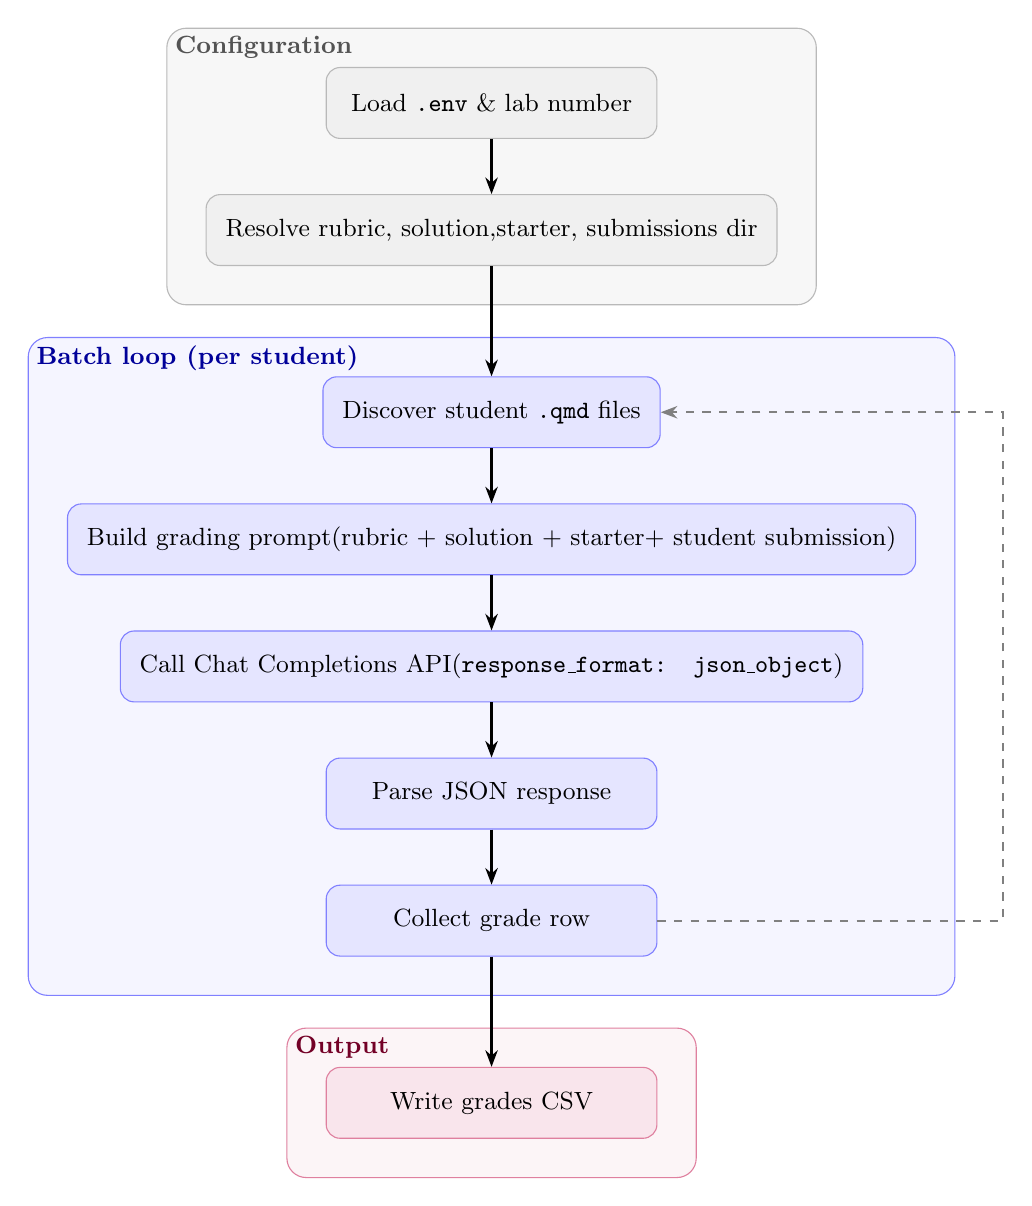
\begin{tikzpicture}[node distance=0.7cm]

%% ---- CONFIGURE ----
\node[config] (env)   {Load \texttt{.env} \& lab number};
\node[config, below=of env] (paths) {Resolve rubric, solution,\\starter, submissions dir};
\draw[arrow] (env) -- (paths);

%% ---- BATCH ----
\node[core,  below=1.4cm of paths] (discover) {Discover student \texttt{.qmd} files};
\node[core,  below=of discover]    (build)    {Build grading prompt\\(rubric + solution + starter\\+ student submission)};
\node[core,  below=of build]       (call)     {Call Chat Completions API\\(\texttt{response\_format: json\_object})};
\node[core,  below=of call]        (parse)    {Parse JSON response};
\node[core,  below=of parse]       (collect)  {Collect grade row};

\draw[arrow] (paths)    -- (discover);
\draw[arrow] (discover) -- (build);
\draw[arrow] (build)    -- (call);
\draw[arrow] (call)     -- (parse);
\draw[arrow] (parse)    -- (collect);

%% loop-back drawn after group boxes so loopbox.east is available

%% ---- OUTPUT ----
\node[outnode, below=1.4cm of collect] (csv) {Write grades CSV};
\draw[arrow] (collect) -- (csv);

%% ---- GROUP BOXES ----
\begin{scope}[on background layer]
  \node[draw=gray!55, fill=gray!6, rounded corners=7pt,
        fit=(env)(paths), inner sep=14pt] (cfgbox) {};
  \node[grouplabel, text=gray!65!black] at (cfgbox.north west) {Configuration};

  \node[draw=blue!50, fill=blue!4, rounded corners=7pt,
        fit=(discover)(build)(call)(parse)(collect), inner sep=14pt] (loopbox) {};
  \node[grouplabel, text=blue!60!black] at (loopbox.north west) {Batch loop (per student)};

  \node[draw=purple!50, fill=purple!4, rounded corners=7pt,
        fit=(csv), inner sep=14pt] (outbox) {};
  \node[grouplabel, text=purple!60!black] at (outbox.north west) {Output};
\end{scope}

%% loop-back: three segments, right angles, routed outside loopbox right edge
\coordinate (rside) at ([xshift=0.6cm]loopbox.east);
\draw[darrow] (collect.east)
  -- (rside |- collect.east)
  -- (rside |- discover.east)
  -- (discover.east);

\end{tikzpicture}
\end{document}
